\documentclass{standalone}
\usepackage{tikz}
\usepackage{pgfornament}
\usetikzlibrary{fit,shapes,positioning,backgrounds}

\begin{document}

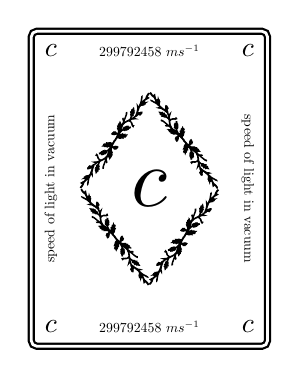
\begin{tikzpicture}[scale=1]
    \def\w{2.5}
    \def\h{3.5}
    \def\k{0.25}
    \def\symbol{$c$}
    \def\name{speed of light in vacuum}
    \def\value{$299792458$}
    \def\unit{$ms^{-1}$}
    \draw[thick,rounded corners=2pt,double=white, double distance =1pt,] (-0.5*\w-\k,-0.5*\h-\k) rectangle (0.5*\w+\k,0.5*\h+\k);
    \path (0.35*\w,0) to [ornament=87] (0,0.35*\h) to [ornament=87]  (-0.35*\w,0) to [ornament=87] (0,-0.35*\h) to [ornament=87] (0.35*\w,0);
    \node[scale=3] (C) at (0,0) {\symbol};
    \node (D1) at (0.5*\w,-0.5*\h) {\symbol};
    \node (D2) at (0.5*\w,0.5*\h) {\symbol};
    \node (D3) at (-0.5*\w,-0.5*\h) {\symbol};
    \node (D2) at (-0.5*\w,0.5*\h) {\symbol};
    \node[scale=0.5] (V1) at (0,0.5*\h) {\value~\unit};
    \node[scale=0.5] (V2) at (0,-0.5*\h) {\value~\unit};
    \node[scale=0.5,rotate=-90] (N1) at (0.5*\w,0) {\name};
    \node[scale=0.5,rotate=90] (N2) at (-0.5*\w,0) {\name};
\end{tikzpicture}

\end{document}
